\documentclass{minimal}

\usepackage{pgf}
\usepackage{tikz}
\usepackage[utf8]{inputenc}
\usetikzlibrary{arrows,automata}
\usetikzlibrary{positioning}


\tikzset{
	state/.style={
		rectangle,
		rounded corners,
		draw=black, very thick,
		minimum height=2em,
		inner sep=2pt,
		text centered,
	},
}

\begin{document}
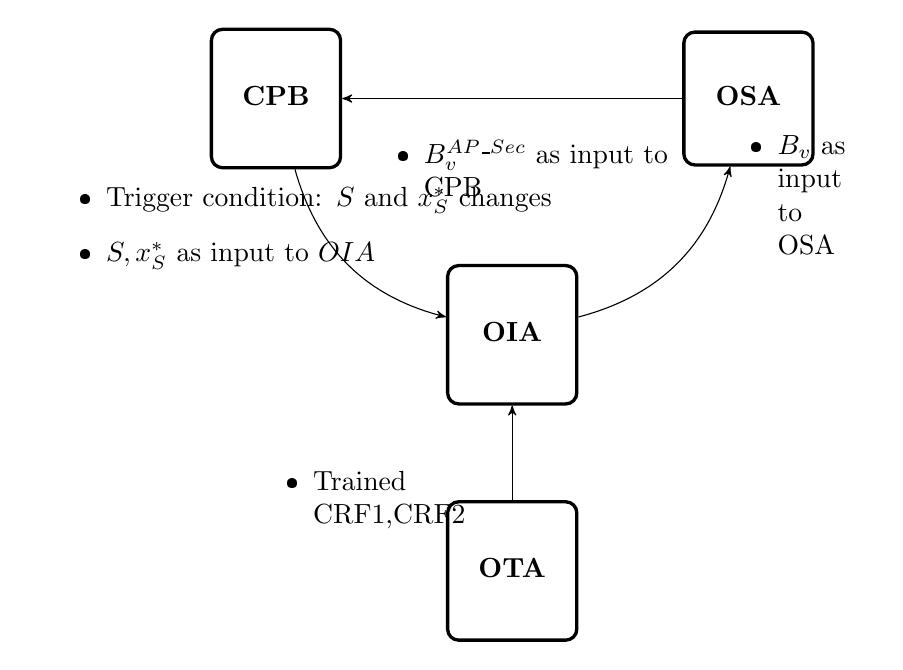
\begin{tikzpicture}[->,>=stealth']

 % First node
 % Use previously defined 'state' as layout (see above)
 % use tabular for content to get columns/rows
 % parbox to limit width of the listing
 \node[state,text width=1.5cm] (CPB) 
 {\begin{tabular}{l}
 	\\[0.5em]
  \textbf{CPB}\\
  \parbox{4cm}{
  }\\[0.5em]
  %\textbf{QueryAdjust}\\
  %\parbox{4cm}{Wähle neue Spreizsequenz}
 \end{tabular}};

 % STATE ACK
 \node[state,
 right of=CPB,
 node distance=6cm,
 %yshift=-4cm,
 text width=1.5cm] (OSA) 
 {	
 \begin{tabular}{l}
 \\[0.4em]
  \textbf{OSA}\\
  \parbox{2.8cm}{ }
  \\[0.4em]
 \end{tabular}

 };

 % STATE OIA
 \node[state,
 below of=OSA,
 xshift=-3cm,
 node distance=3cm,text width=1.5cm] (OIA) 
 {%
 \begin{tabular}{l}
 \\[0.5em]
  \textbf{OIA}\\
  %\parbox{4cm}{Produktcode entspreizen und erfassen}
  \\[0.5em]
 \end{tabular}
 };
 
 %OTA
 \node[state,
 below of=OIA,
 node distance=3cm,text width=1.5cm] (OTA) 
 {%
 	\begin{tabular}{l}
 	\\[0.5em]
 	\textbf{OTA}\\
 	%\parbox{4cm}{Produktcode entspreizen und erfassen}
 	\\[0.5em]
 	\end{tabular}
 };
 
 
 % draw the paths and and print some Text below/above the graph
 \path 
 (OIA)  edge[bend right=30]   node[anchor=south,above,text width=2cm,xshift=4em]
 {
 	\begin{itemize}
 	\item $B_{v}$ as input to OSA
 	\end{itemize}
 }         (OSA)
 
 (CPB)  edge [bend right=30] node[anchor=east,left,text width=7cm,xshift=9em,yshift=2em]
                  {
                  \begin{itemize}
                   \item Trigger condition: $S$ and $x_{S}^{*}$ changes
                   \item $S,x_{S}^{*}$ as input to $OIA$
                  \end{itemize}
                  } (OIA)

 (OSA)  edge[bend left=0] node[anchor=north,below,text width=4cm]
                  {\begin{itemize}
                   \item $B_{v}^{AP\_Sec}$ as input to CPB
                  \end{itemize}
                  } (CPB)
(OTA)  edge[bend left=0] node[anchor=north,below,text width=4cm,xshift=-4em,yshift=1em]
{\begin{itemize}
	\item Trained CRF1,CRF2
	\end{itemize}
} (OIA)                  
 ;
\end{tikzpicture}
\end{document}